% \listoftodos

\chapter{Least trimmed squares}
In this chapter, we introduce one of the most common regression analysis models which is known as the linear regression model. It aims to model the relationship between one variable which is called \defterm{dependent} and one or more variables which are called \defterm{explanatory}. The relationship is based on a model function with parameters which are not known in advance and are to be estimated from data. We also describe one of the most common methods for finding those parameters in this model, namely the ordinary least squares method. It is important to note that all vectors in this text are considered as column vectors. On the other hand, we denote a row vector as a transposed vector.



%%%%%%%%%%%%%%%%%%%%%%%%%%%%%%%%%%%%%%%%%%%%%%%%%%%%%%%%%%%%%%%%%%%%%%%%%%%%%%%%%%%%%%%%%%%%%%%%%%%%
%%%%%%%%%%%%%%%      SECTION: LINEAR REGRESSION MODEL     %%%%%%%%%%%%%%%%%%%%%%%%%%%%%%%%%%%%%%%%%%
%%%%%%%%%%%%%%%%%%%%%%%%%%%%%%%%%%%%%%%%%%%%%%%%%%%%%%%%%%%%%%%%%%%%%%%%%%%%%%%%%%%%%%%%%%%%%%%%%%%%

\section{Linear regression model}
\begin{definition}\label{definition:lr_model}
    The \defterm{linear regression model} is given by
\begin{equation}
        y = \vec{x}^T\vec{w} + \varepsilon ,
\end{equation}
where $y \in \mathbb{R}$ is a random variable which is called \defterm{dependent variable} and $\vec{x}^T = (x_1, x_2, \ldots, x_p)$ is a vector of \defterm{explanatory variables}. Usually we call $x_i$ a regressor. Finally $\varepsilon \in \mathbb{R}$ is a random variable called \defterm{noise} or \defterm{error}. The vector $\vec{w} = (w_1, w_2, \ldots, w_p)$ is a vector of parameters called  \defterm{regression coefficients}. 
\end{definition}
In regression analysis we aim to estimate the $\vec{w}$ using $n$ measurements of $y$ and $\vec{x}$. We can write this in matrix form 

% In practice, we usually deal with multiple dependent variables so we define multiple linear regression model.

% \begin{definition}\label{definition:lr_model_multiple}
% The \defterm{multiple linear regression model} is 
% \begin{equation}
%         y_i = \vec{x_i}^T\vec{w} + \varepsilon_i,\\ i=1,\ldots , n.
% \end{equation}
% It is common to write the whole model in a matrix form

\begin{equation}
    \vec{y} = \vec{X}\vec{w} + \vec{\varepsilon}    \numberthis
\end{equation} where

\[ 
\vec{y} = \begin{bmatrix}
    y_{1} \\
    y_{2} \\
    \vdots \\
    y_{n}
  \end{bmatrix}\\,
 \vec{X} = \begin{bmatrix}
    \vec{x_1}^T \\
    \vec{x_2}^T \\
    \vdots \\
    \vec{x_n}^T
\end{bmatrix}
=
\begin{bmatrix}
    x_{11} & x_{12} & x_{13} & \dots  & x_{1p} \\
    x_{21} & x_{22} & x_{23} & \dots  & x_{2p} \\
    \vdots & \vdots & \vdots & \ddots & \vdots \\
    x_{n1} & x_{n2} & x_{n3} & \dots  & x_{np}
\end{bmatrix}\\,
\vec{w} = \begin{bmatrix}
    w_{1} \\
    w_{2} \\
    \vdots \\
    w_{p}
  \end{bmatrix}\\,
  \vec{\varepsilon} = \begin{bmatrix}
    \varepsilon_{1} \\
    \varepsilon_{2} \\
    \vdots \\
    \varepsilon_{n}
  \end{bmatrix}
\]
This means that we can think of rows of matrix $\vec{X}$ as columns vectors $\vec{x_i}$ written into the row.

It is assumed that errors are independent and identically distributed so that $\vec{\varepsilon} \sim \mathcal{N}(0,\,\sigma^{2})$.
% \end{definition}
%It this work we talk about the multiple linear regression model, but for simplicity, we call it merely the linear regression model.

\begin{note}
    It is usual refer to given $\vec{X}$ and $\vec{y}$ as to \defterm{data set} and to $y_i$ with corresponding $\vec{x_i}$ as to $i$th \defterm{data sample} or \defterm{observation}.
\end{note}

%%%% OK TO HERE
\subsection{Prediction with the linear regression model}
The linear regression model contains the vector $\vec{w}$ of regression coefficients which are unknown and which we need to estimate in order to be able to use the model for predictions. Let us assume that we already have estimated regression coefficients as $\vec{\hat{w}}$. Then the predicted values of $y$ are given by
\begin{equation}
    \hat{y} = \vec{\hat{w}}^T\vec{x}. \numberthis
\end{equation}
The true value of $y$ is given by 
\begin{equation}
    y = \vec{w^{*}}^T\vec{x} + \varepsilon
\end{equation}
where $ \vec{w^{*}}$  represents actual regression coefficients which we aim to estimate. 

Because we assume linear dependence between dependent variable $y$ and explanatory variables $\vec{x}$ which we assume to be non-random, then what makes $y$ random variable is a random variable $\varepsilon$. Because we assume that $\mathbb{E}(\varepsilon) = 0$ we can see that 

\begin{equation} \label{equation:vary}
\mathbb{E}(y) = \vec{x}^T\vec{w} + \mathbb{E}(\varepsilon) = \vec{x}^T\vec{w}
\end{equation}
so $\hat{y}$ is a point estimation of the expected value of $y$.

\subsubsection*{Intercept}
In real world situations it is not usual that $\mathbb{E}(\varepsilon) = 0$. Consider this trivial example.
\begin{example} \label{example:intercept}
Let us consider that $y$ represents price of the room and $x$ represents the number of the windows in such a room. If this room does not have windows thus $x = 0$ and $\mathbb{E}(\varepsilon) = 0$ then $ y = wx + \varepsilon$ equals zero. But it is very unlikely that room without windows is free. 
\end{example}

Because of that, it is very common to include one constant regressor $x_1 = 1$. The corresponding coefficient $w_1$ of $\vec{w}$ is called an \defterm{intercept}. We refer this model as a \defterm{model with an intercept}. The intercept then corresponds to expected value of $y$ when all regressors are zero and prevent the problem from Example~\ref{example:intercept}. This means that intercept can be assumed as a shift so that it corresponds to $\mathbb{E}(\varepsilon) = \mu$. With regards to this fact we can still assume that in the model with intercept $\varepsilon \sim \mathcal{N}(0,\,\sigma^{2})$.
In this work, we consider the model with the intercept. This means that we consider $\vec{x} = (x_1, x_2 \ldots x_p)$ where constant $x_1 = 1$ represents intercept.  
\begin{note}
Sometimes in the model with an intercept, the explanatory variable $\vec{x}$  is marked as $\vec{x} \in \mathbb{R}^{p+1}, \vec{x} = (x_0, x_1 \ldots x_p)$, 
which means that actual observation $\vec{x} \in \mathbb{R}^p$ and the intercept $x_0 = 1$ is explicitly marked.
\end{note} 


%%%%%%%%%%%%%%%%%%%%%%%%%%%%%%%%%%%%%%%%%%%%%%%%%%%%%%%%%%%%%%%%%%%%%%%%%%%%%%%%%%%%%%%%%%%%%%%%%%%%
%%%%%%%%%%%%%%%      SECTION: ORDINARY LEAST SQUARES    %%%%%%%%%%%%%%%%%%%%%%%%%%%%%%%%%%%%%%%%%%%%
%%%%%%%%%%%%%%%%%%%%%%%%%%%%%%%%%%%%%%%%%%%%%%%%%%%%%%%%%%%%%%%%%%%%%%%%%%%%%%%%%%%%%%%%%%%%%%%%%%%%

\section{Ordinary least squares}
We want to estimate $\vec{w}$ so that an error of the model on the whole data set is the least possible. This error is measured by a \defterm{loss function} 
$L : \mathbb{R}^2 \rightarrow  \mathbb{R}$,
which in case of the \defterm{ordinary least squares} (OLS) method is quadratic loss function $L(y, \hat{y}) := (y - \hat{y})^2$. 
So the idea is to find $\vec{\hat{w}}$ so that it minimizes the sum of squared \defterm{residuals}
\begin{equation}
    r_i(\vec{w}) =y_i - \hat{y_i} = y_i - \vec{x_i}^T\vec{w} ,\ i = 1,2,\ldots ,n.
\end{equation}
This is commonly know as residual sum of squares $RSS$
\begin{equation}
    RSS(\vec{w}) = \sum\limits_{i=1}^n r_i^2(\vec{w}) = \sum\limits_{i=1}^n (y_i - \vec{w}^T\vec{x_i})^2.
\end{equation}
\begin{definition} The RSS as the function of $\vec{w}$ is an \defterm{objective function} for OLS
    \begin{equation}
        \of^{(OLS,\vec{X}, \vec{y})}(\vec{w}) = \sum\limits_{i=1}^n (y_i - \vec{w}^T\vec{x_i})^2 = (\vec{Y} - \vec{X}\vec{w})^T(\vec{Y} - \vec{X}\vec{w}).
    \end{equation}
\end{definition}
The point of the minimum of this function 
\begin{equation}
\vec{\hat{w}}^{(OLS,\vec{X}, \vec{y})}  = \argmin_{\vec{w} \in \mathbb{R}^p} \of^{(OLS,\vec{X}, \vec{y})}(\vec{w})
\end{equation}
is a the ordinary least squares estimate of regression coefficients.

To find the minimum of this function, we first need to find the gradient by calculating all partial derivatives
\begin{equation}
    \frac{\partial {\of^{(OLS,\vec{X}, \vec{y})}} }{\partial w_j} = \sum\limits_{i=1}^n 2(y_i - \vec{w}^T\vec{x_i})(-x_{ij}) \\, \ \ j \in \{{1,2,\ldots,p\}}. 
\end{equation}
By this we obtain the gradient 
\begin{equation}
    \nabla \of^{(OLS,\vec{X}, \vec{y})} = -\sum\limits_{i=1}^n 2(y_i - \vec{w}^T\vec{x_i})\vec{x_i}. 
\end{equation}
Putting gradient equal to zero we get the so called \defterm{normal equations}
\begin{equation}
    -\sum\limits_{i=1}^n 2(y_i - \vec{w}^T\vec{x_i})\vec{x_i} = 0 
\end{equation}
that can be rewritten in a matrix form as 
\begin{equation}    \label{equation:zerogradient}
    \vec{X}^T\vec{y} - \vec{X}^T\vec{X}\vec{w} = 0.
\end{equation}

Let us now construct the hessian matrix using second-order partial derivatives:
\begin{equation}
    \frac{\partial^2{\of^{(OLS,\vec{X}, \vec{y})}} }{\partial w_h\partial w_j} = \sum\limits_{i=1}^n 2(- x_{ik})(-x_{ij}) \\, \ \ h \in \{{1,2,\ldots,p\}}. 
\end{equation}
We get 
\begin{equation}
    \vec{H_{\of^{(OLS,\vec{X}, \vec{y})}}} = 2\vec{X}^T\vec{X}.
\end{equation}

We can see that hessian $\vec{H_{\of^{(OLS,\vec{X}, \vec{y})}}}$ is always positive semi-definite because for all $\vec{s} \in \mathbb{R}^p$

\begin{equation}
    \vec{s}^T(2\vec{X}^T\vec{X})\vec{s} = 2(\vec{X}\vec{s})^T(\vec{X}\vec{s}) =  2 \norm{\vec{X}\vec{s}}^2
\end{equation}

It is easy to prove that twice differentiable function is convex if and only if the hessian of such function is positive semi-definite. Moreover, any local minimum of the convex function is also the global one. Hence the solution of~\eqref{equation:zerogradient} gives us the global minimum. 

Assuming that $\vec{X}^T\vec{X}$ is a regular matrix, its inverse exists, and the solution can be explicitly written as

\begin{equation} \label{wols}
    \vec{\hat{w}}^{(OLS,\vec{X}, \vec{y})} = (\vec{X}^T\vec{X})^{-1}\vec{X}^T\vec{y}.
\end{equation}
%where $(OLS,n)$ denotes that $\vec{\hat{w}}^{(OLS,n)}$ is the estimate of true regression coefficients given by the OLS method for $n$ observations. 

Moreover, we can see that if $\vec{X}^T\vec{X}$ is a regular matrix, then the hessian $\vec{H_{\of^{(OLS,\vec{X}, \vec{y})}}}$ is positive definite and $\of^{(OLS,\vec{X}, \vec{y})}$ is strictly convex and $\vec{\hat{w}}^{(OLS,\vec{X}, \vec{y})}$ is the unique strict global minimum.

% norms can be used to create distance as d(x,y) = || x - y ||
% but not all distances have corresponding norm! trivial example. d(x,x) = 0, d(x,y) = 1

\subsection{Properties of the OLS estimate}
Gauss-Markov theorem~\cite{mccullagh2018generalized} tells us that if particular assumptions about the regression model are fulfilled then the OLS estimate is unbiased and efficient. Gauss-Markov theorem states that OLS is the best linear unbiased estimator (BLUE). Being an efficient estimate means that any other linear unbiased estimate has the same or higher variance. The most important conditions are:

\begin{itemize} \label{ols:assumptions}
  \item Expected value of errors is zero.
  \item Errors are independently distributed and uncorrelated thus \\ $cov(\varepsilon_i, \varepsilon_j), \ i, j = 1, 2 \ldots , n, \ \ i \neq j$
 % \item Regressors $\vec{x_i}, i = 1, 2, \ldots , n$ and corresponding errors 
%$\varepsilon_i, \ i = 1,2, \ldots , n$ are uncorrelated.
 \item All errors have same finite variance. This is known as \defterm{homoscedasticity}.
\end{itemize}

% \begin{note}
%  As described in Example~\ref{example:intercept} the first assumption is usually fulfilled if we use the model with intercept. Rest of the conditions, on the other hand, are rarely met.
% \end{note}

There are also other theorems which describe properties of OLS under specific conditions, but they are out if the scope of this work.


%%%%%%%%%%%%%%%%%%%%%%%%%%%%%%%%%%%%%%%%%%%%%%%%%%%%%%%%%%%%%%%%%%%%%%%%%%%%%%%%%%%%%%%%%%%%%%%%%%%%
%%%%%%%%%%%%%%%      SECTION: ROBUST STATISTICS      %%%%%%%%%%%%%%%%%%%%%%%%%%%%%%%%%%%%%%%%%%%%%%%
%%%%%%%%%%%%%%%%%%%%%%%%%%%%%%%%%%%%%%%%%%%%%%%%%%%%%%%%%%%%%%%%%%%%%%%%%%%%%%%%%%%%%%%%%%%%%%%%%%%%

\section{Robust statistics} \label{section:roboust}
Standard statistics methods rely on multiple assumptions and fail if those assumptions are not met. The goal of the robust statistics is to produce acceptable results even when the data are from some unconventional distributions or if data contains outliers or errors which are not normally distributed. 

Such assumptions about the OLS method are described in Section~\ref{ols:assumptions}. Before we explain what happens if those conditions are not met or met only partially let us describe one of the most common reasons why assumptions are false.

\subsection{Outliers} \label{outliers:info}
We stated many assumptions that are required for the OLS method to produce a acceptable estimate of $\vec{\hat{w}}$. Unfortunately, in real conditions, these assumptions are often false so that the ordinary least squares do not guarantee to return reasonable results. One of the most common reasons for the assumptions being not met are observations called outliers.

Outliers are for instance erroneous measurements such as transmission errors or noise. Another common reason for outliers is that nowadays the data are automatically processed by computers. Sometimes we are also given data which are heterogeneous in the sense that they contain data from multiple regression models. In some sense outliers are inevitable. One would say that we should be able to eliminate them by precise examination, repair or removal of such data. That is possible in some cases, but often the data we are dealing with are too big and highly dimensional to check.

The robust methods are sometimes not only useful to create models that are not being unduly affected by the presence of outliers but also capable of identifying data which seems to be outliers. 

We use terminology from~\cite{rouss:1990} to describe certain types of outliers. Let us have observation $(y_i, \vec{x_i})$. If the observation is not outlying in any direction we call it \defterm{regular observation} . If it is outlying in direction of the explanatory variable $\vec{x_i}$  we call it \defterm{leverage point}. We have two types of leverage points. If $\vec{x_i}$ is outlying but $(y_i, \vec{x_i})$ follows the liner pattern we call it a \defterm{good leverage point}. If it does not follow such a pattern we call it \defterm{bad leverage point}. Finally if $(y_i, \vec{x_i})$ is  outlying only in direction of $y_i$, we call it a \defterm{vertical outlier}.

\subsection{Measuring robustness}
There are a couple of tools to measure the robustness of an estimate. One of the most popular one is called \defterm{breakdown point}. Others are \defterm{empirical influence function} and \defterm{influence function and sensitivity curve}.  Here we describe only breakdown point right now. More on robustness measures can be found in~\cite{hampel1986robust}.

\begin{definition}
    Let $T$ be a statistics, $\vec{x} = (x_1, x_2,\ldots,x_n)$ be an $n$-element random sample and $T_n(\vec{x})$ value of this statistics. The breakdown point of $T$ at sample $\vec{x}$ is defined using sample $\vec{\overline{x}}^{(k)}$, that arose by replacing $k$ points from the original sample $\vec{x}$ with random values $x_i$. Then the \defterm{breakdown point} is 

\begin{equation}
    \bdpoint(T,\vec{x_n} ) = \frac{1}{n} \min S_{T, \vec{x_n}} , 
\end{equation}
where 
\begin{equation}
   S_{T, \vec{x_n}, D} = 
  \left\{ k \in \{{1,2, \ldots ,n\}} : \sup_{ \vec{\overline{x}}^{(k)} } \norm{T_n(\vec{x}) - T_n(\vec{\overline{x}}^{(k)})} = \infty   \right\}.  
\end{equation}
\end{definition}

This definition is says that the breakdown point is the function of the minimal number of observations needed to be changed so that the estimator gives arbitrarily biased results.

Intuitively, a reasonable breakdown point should not be higher than~$0.5$~\cite{rouss:1986} ; if more than $50\%$ of the data is exchanged, the model of exchanged data should override the model of the original data. 

In the case of the OLS estimator, one outlier is enough to increase the value of $\vec{\hat{w}}^{(OLS,\vec{X}, \vec{y})}$ to any desired value~\cite{agullo2001new} thus 
\begin{equation}
    \bdpoint(\vec{\hat{w}}^{(OLS,\vec{X}, \vec{y})},\vec{x_n} ) = \frac{1}{n}.
\end{equation}

\begin{figure}[h]
    \centering
    % \missingfigure{Image visualizing  one C-step}
    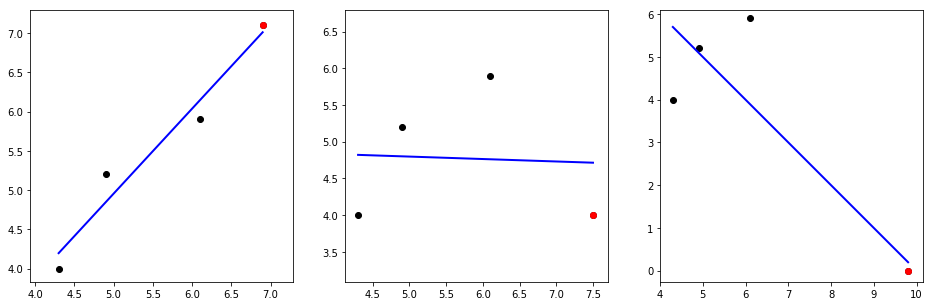
\includegraphics[width=12cm]{img/outlier_regression}
    \caption{Change of the regression hyperplane given by coefficients estimated with OLS method when one of the four observations (highlighted with red color) starts to deviate from the linear pattern.}
    \label{figure:outlier:hyperplane}
\end{figure}

Figure~\ref{figure:outlier:hyperplane} gives us an idea of how one outlier may change the hyperplane given by the OLS estimator of regression coefficients.



    

For an increasing number of the data samples $n$ the breakdown point of $\vec{\hat{w}}^{(OLS,\vec{X}, \vec{y})}$ tends to zero. We can see that ordinary least squares estimator is not resistant to outliers at all. Due to this fact, multiple robust estimators alternatives to the OLS have been proposed.




%%%%%%%%%%%%%%%%%%%%%%%%%%%%%%%%%%%%%%%%%%%%%%%%%%%%%%%%%%%%%%%%%%%%%%%%%%%%%%%%%%%%%%%%%%%%%%%%%%%%
%%%%%%%%%%%%%%%      SECTION: LEAST TRIMMED SQUARES       %%%%%%%%%%%%%%%%%%%%%%%%%%%%%%%%%%%%%%%%%%
%%%%%%%%%%%%%%%%%%%%%%%%%%%%%%%%%%%%%%%%%%%%%%%%%%%%%%%%%%%%%%%%%%%%%%%%%%%%%%%%%%%%%%%%%%%%%%%%%%%%
\section{Least trimmed squares}
The least trimmed squares (LTS) estimator is a robust version of the OLS estimator. In this section, we give a definition and show that its breakdown point is variable and can go up to the maximum possible value of breakdown point, thus~$0.5$.

\begin{definition} \label{definition:of:lts:real}
Let us have $\vec{X} \in \mathbb{R}^{n,p}$, $\vec{y} \in \mathbb{R}^{n,1}$, 
    $\vec{w} \in \mathbb{R}^p$ and $h$, $ n/2 \leq h \leq n$. The objective function of LTS for data $\vec{X}$ and $\vec{y}$ is
    \begin{equation}  
        \of^{(LTS,h, n)}(\vec{w}) =  \sum\limits_{i=1}^h r_{i:n}^2(\vec{w})  
    \end{equation}
\end{definition}
where $r_{i:n}^2(\vec{w})$ denotes the $i$th smallest squared residuum at $\vec{w}$, i.e. 
\begin{equation}
    r_{1:n}^2(\vec{w}) \leq r_{2:n}^2(\vec{w}) \leq \ldots \leq r_{n:n}^2(\vec{w}).   
\end{equation} 

Even though that objective function of LTS seems similar to the OLS objective function, finding the minimum is far more complex because the order of the least squared residuals depends on $\vec{w}$. Moreover, $r_{i:n}^2(\vec{w})$ residuum is not uniquely determined if more squared residuals have same value. This makes finding the LTS estimate non-convex optimization problem and, in fact, finding the global minimum is NP-hard~\cite{bernholt2006robust}. 

\subsection{Discrete objective function} \label{sectionofltsdiscrete}
The LTS objective function from Definition~\ref{definition:of:lts:real} is not differentiable and not convex, so we are unable to use the same approach as with the OLS objective function. Let us transform this objective function to a discrete version which is easier to use by algorithms to minimize it.

Let us assume for now that we know the vector $\vec{\hat{w}}^{(LTS,h, n)}$ of estimated regression coefficients minimizing the LTS objective function. Let $\pi$ be the permutation of $\hat{n} = \{{1,2,\ldots, n\}}$ such that 

\begin{equation}
    r_{i:n}(\vec{\hat{w}}^{(LTS,h, n)}) = r_{\pi(j)}(\vec{\hat{w}}^{(LTS,h, n)})\\, \ \ j \in \hat{n}.
\end{equation}
Put
 \begin{equation}
   Q^{(n,h)} = \left\{ \vec{m} \in \mathbb{R}^n \ | \ m_i \in \{{0, 1\}} \\,i \in \hat{n} \\,   \sum\limits_{i=1}^n  m_i = h \right\},
\end{equation}
which is simply the set of all vectors $\vec{m} \in \mathbb{R}^n$ which contain $h$ ones and $n-h$ zeros. Let $\vec{m}^{(LTS)} \in Q^{(n,h)}$  such that  $m^{(LTS)}_j = 1$ when $\pi(j) \leq h$ and $m^{(LTS)}_j = 0$ otherwise. Then

\begin{equation} \label{ltshat}
    \vec{\hat{w}}^{(LTS,h, n)} =  
  \argmin_{\vec{w} \in \mathbb{R}^p} \sum\limits_{i=1}^h r_{i:n}^2(\vec{w}) = 
  \argmin_{\vec{w} \in \mathbb{R}^p} \sum\limits_{i=1}^n m^{(LTS)}_i r_{i}^2(\vec{w}). 
\end{equation}
This means that if we know the vector $\vec{m}_{LTS}$ than we can compute the LTS estimate as the OLS estimate with $\vec{X}$ and $\vec{Y}$ multiplied by the diagonal matrix $\vec{M}_{LTS} = diag(\vec{m}^{(LTS)})$:

\begin{equation}  \label{lts:discrete:objective}
    \vec{\hat{w}}^{(LTS,h, n)} = (\vec{X}^T\vec{M}_{LTS}\vec{X})^{-1}\vec{X}^T\vec{M}_{LTS}\vec{y}.
\end{equation}
In other words, finding the minimum of the LTS objective function can be done by finding the OLS estimates~\eqref{lts:discrete:objective} for all vectors 
$\vec{m} \in Q^{(n,h)}$. 
Thus, as described in~\cite{kloudaVyzkumnyUkol},


% {(LTS,\vec{X_{M}}, \vec{y_{M}} }(\vec{m})


\begin{align} \label{kloudaodvozeni}
\minim_{\vec{w} \in \mathbb{R}^p} 
    \of^{(LTS,h, n)}(\vec{w})  
&=\minim_{\vec{w} \in \mathbb{R}^p} 
    \sum\limits_{i=1}^h r_{i:n}^2(\vec{w})  \\
&= \minim_{\vec{w} \in \mathbb{R}^p,\vec{m} \in Q^{(n,h)}} 
        \sum\limits_{i=1}^n m_i r_{i}^2(\vec{w})\\
&= \minim_{\vec{m} \in Q^{(n,h)}} 
            \Big( \minim_{\vec{w} \in\mathbb{R}^p} 
            \of^{(OLS,\vec{M}\vec{X},  \vec{M}\vec{y} )} (\vec{w}) \Big)\\
&= \minim_{\vec{m} \in Q^{(n,h)}} 
            \Big(\minim_{\vec{w} \in\mathbb{R}^p}  
            \norm{ \vec{M}\vec{y} -   \vec{M}\vec{X}\vec{w}  }^2 \Big).
\end{align}

Substituting $\vec{w}$ with the OLS estimate as in~\eqref{ltshat} we get
% %% TODO %%%%%%%%%%%%%%%%%%%%%%%%%%%%%%
% \begin{align*}
% \vec{\hat{w}}^{(LTS,h, n)}
% &=  \minim_{\vec{m} \in Q^{(n,h)}} 
%     \Big( \norm{ \vec{M}\vec{y} -  \vec{M}\vec{X}(\vec{X}^T\vec{M}\vec{X})^{-1}\vec{X}^T\vec{M}\vec{y}  }^2 \Big)
% \end{align*}
the discrete objective function with domain $\vec{m} \in Q^{(n,h)}$

\begin{equation} \label{oflts_discrete}
    \oflts(\vec{m}) =  \norm{ \vec{M}\vec{y} -  \vec{M}\vec{X}(\vec{X}^T\vec{M}\vec{X})^{-1}\vec{X}^T\vec{M}\vec{y}  }^2.
\end{equation}

Minimizing this OF could by done straightforwardly by iterating over the $Q^{(n,h)}$ set. Unfortunately, this set has cardinality equal to $\binom{n}{h}$, which is huge, so this approach is infeasible for bigger data sets. Multiple algorithms were proposed to overcome this problem. Majority of them are probabilistic algorithms, but besides those, some exact algorithms were proposed. 

Finally, let us point out some fact about the number $h$ of non-trimmed residuals and how it makes least trimmed squares robust.
The LTS reaches maximum breakdown point $0.5$ at $h = [(n/2] + [(p+1)/2]$~\cite{agullo2001new}.
This means that up to $50\%$ of the data can be outliers. In practice, the portion of outliers is usually lower; if an upper bound on the percentage of outliers is known,  $h$ should be set to match this percentage.